\normaltrue \difficilefalse \tdifficilefalse
\correctiontrue

%\UPSTIidClasse{11} % 11 sup, 12 spé
%\newcommand{\UPSTIidClasse}{11}

\exer{Diagramme de Bode$\star$ \label{C2:02:510_01}}
\setcounter{numques}{0}
\UPSTIcompetence[2]{C2-02}
\index{Compétence C2-02}
\index{Diagramme de Bode}
\ifcorrection
\else
\textbf{Pas de corrigé pour cet exercice.}
\fi

 
\question{Tracer le diagramme de Bode de la fonction de transfert suivante : $F_1(p)=\dfrac{15}{1+10p}$.}

\ifprof
\textbf{Tracer asymptotique}

\begin{center}

\includegraphics[width=.9\linewidth]{tab_01}
\end{center}


\textbf{Positionnement du diagramme de gain}
Lorsque que $\omega$ tend vers 0, le gain tend vers $20 \log 15 = \SI{23,5}{dB}$.


\begin{center}
\begin{tikzpicture}[xscale=2]
\tikzset{
semilog lines/.style={thin, bleuxp}, 
semilog lines 2/.style={semilog lines,bleuxpc},
semilog half lines/.style={semilog lines 2,dotted },
semilog label x/.style={semilog lines,below,font=\tiny,black},
semilog label y/.style={semilog lines,right,font=\tiny,black}
}

\begin{scope}[yscale=1/20]
\semilog{-3}{1}{-30}{30}

\BodeAmp[orangexp,thick,samples=100]{-3:1}{\POAmpAsymp{15.}{10.}}
\BodeAmp[orangexp,ultra thick]{-3:1}{\POAmp{15}{10}}

\BodeGraph[orangexp,thin,samples=100]{-3:1}{\POAmpAsymp{15}{1}}
%\BodeGraph{-2:2}{\POAmp{6}{0.3}}

\draw (-2.2,27) node {\footnotesize 23,5 dB, 0 dB/d\'ecade};
\draw (.3,15) node {\footnotesize $-$20 dB/d\'ecade};
\draw [dashed,ultra thick,bleuxp] (-1,-1) -- (-1,23.5);
\draw (-1,-1)  node {\Huge $\cdot$} node [above right]{\footnotesize 0,1};
\end{scope}
\begin{scope}[yshift=-3cm,yscale=1/90]
\UniteDegre
\OrdBode{45}
\semilog{-3}{1}{-180}{90}
\BodeArg[orangexp,samples=200,thick]{-3:1}{\POArgAsymp{15.}{10.}}
\BodeArg[orangexp,ultra thick]{-3:1}{\POArg{15}{10}}
\end{scope}
\end{tikzpicture}
\end{center}

\begin{tikzpicture}[xscale=7/4]
\begin{scope}[yscale=3/40]
\semilog{-2}{2}{-20}{20}
\BodeGraph{-2:2}{\POAmpAsymp{6}{0.3}}
\BodeGraph{-2:2}{\POAmp{6}{0.3}}
\end{scope}

\end{tikzpicture}


%\begin{center}
%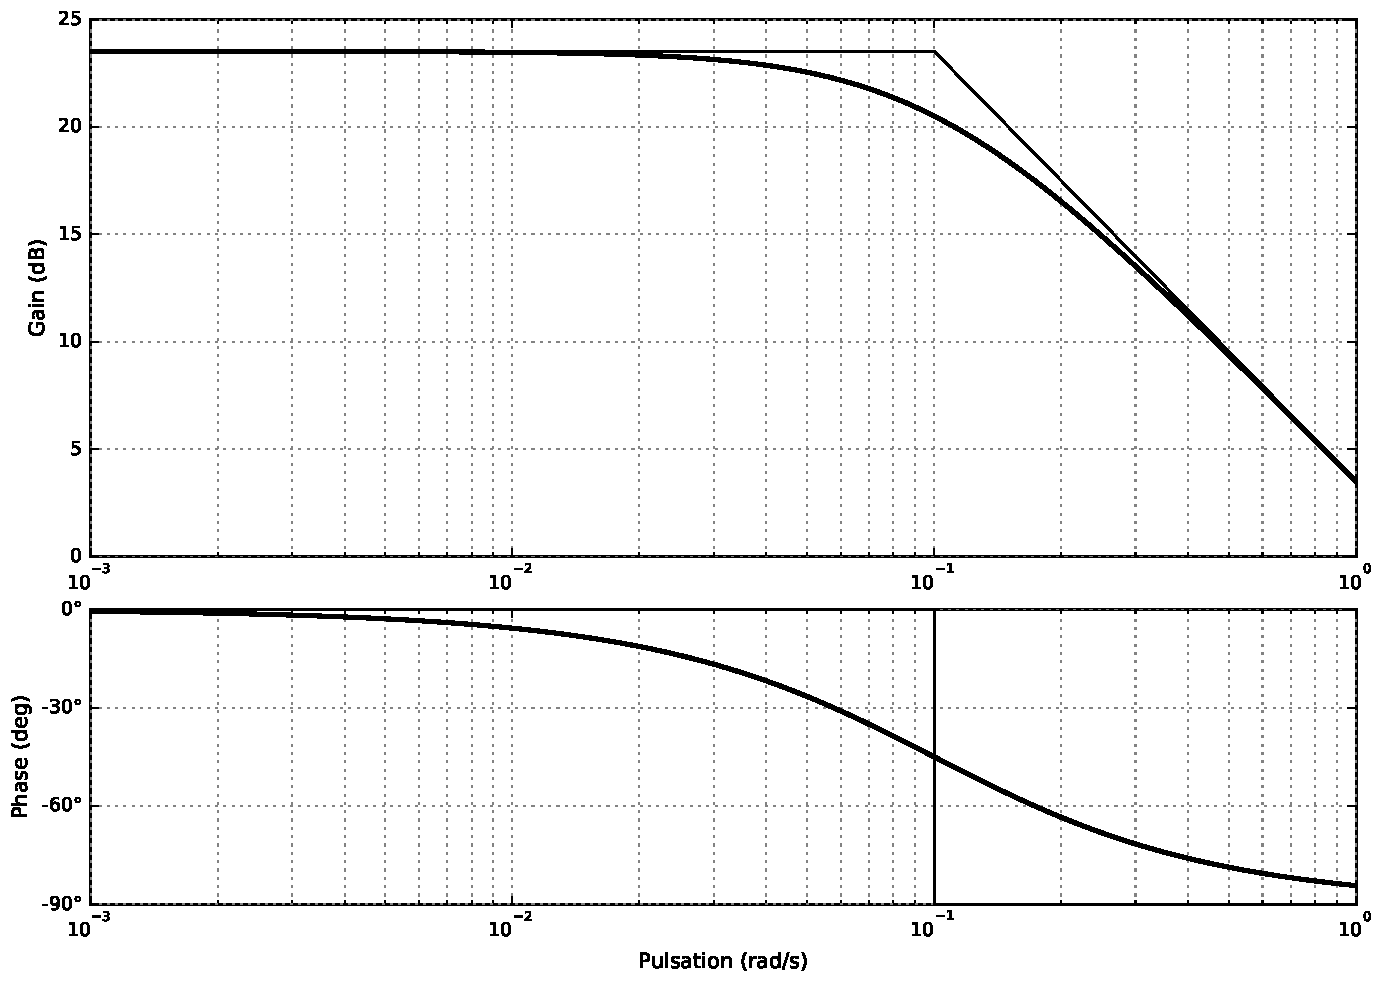
\includegraphics[width=.9\linewidth]{bode_01}
%\end{center}

\else 


\fi

\question{Le système est sollicité par une entrée sinusoïdale de période \SI{6}{s} et d'amplitude 10. Quel est le signal de sortie ?}
\ifprof
Pour une période de \SI{60}{s}, la pulsation est de $\dfrac{2\pi}{T}$ soit $\omega = \SI{0,1}{rad.s^{-1}}$.
Pour cette pulsation le gain est de \SI{20}{dB} et le déphasage de $-\dfrac{\pi}{4}$.

On a donc $20\log(S/E) = 20$ soit $S=10E$. Le signal d'entrée est donc $e(t) = 10 \sin (0,1 t)$ et le signal de sortie  $s(t) = 100 \sin\left(0,1 t - \dfrac{\pi}{4}\right)$.
\else
\fi

\ifprof
\else
\begin{flushright}
\footnotesize{Corrigé  voir \ref{C2:02:510_01}.}
\end{flushright}%
\fi